\documentclass[
    % -- opções da classe memoir --
    article,			% indica que é um artigo acadêmico
    11pt,				% tamanho da fonte
    oneside,			% para impressão apenas no recto. Oposto a twoside
    a4paper,			% tamanho do papel. 
    % -- opções da classe abntex2 --
    %chapter=TITLE,		% títulos de capítulos convertidos em letras maiúsculas
    %section=TITLE,		% títulos de seções convertidos em letras maiúsculas
    %subsection=TITLE,	% títulos de subseções convertidos em letras maiúsculas
    %subsubsection=TITLE % títulos de subsubseções convertidos em letras maiúsculas
    % -- opções do pacote babel --
    english,			% idioma adicional para hifenização
    brazil,				% o último idioma é o principal do documento
    sumario=tradicional
]{abntex2}

% Pacotes
% -----
% Pacotes fundamentais 
% -----
\usepackage{lmodern}			% Usa a fonte Latin Modern
\usepackage[T1]{fontenc}		% Seleção de códigos de fonte.
\usepackage[utf8]{inputenc}		% Codificação do documento (conversão automática dos acentos)
\usepackage{indentfirst}		% Identa o primeiro parágrafo de cada seção.
\usepackage{nomencl} 			% Lista de símbolos
\usepackage{color}				% Controle das cores
\usepackage{graphicx}			% Inclusão de gráficos
\usepackage{microtype} 			% Para melhorias de justificação
\usepackage[brazilian,hyperpageref]{backref}	 % Páginas com as citações na bibliografia
\usepackage[subentrycounter,seeautonumberlist,nonumberlist=true,acronym,nohypertypes={index}]{glossaries} % Glossário. Deve ser carregado depois de backref
\usepackage[alf]{abntex2cite}	% Citações padrão ABNT. Deve ser carregado depois de glossaries
\usepackage[portuguese]{todonotes}
\usepackage{multirow}
\usepackage{longtable}
% -----

% -----
% Configurações dos pacotes
% -----

% --- Glossaries ---
\newglossary[ilg]{index}{ind}{idx}{\indexname}
\newcommand*{\newterm}[2]{
    \newglossaryentry{#1}
    {type=index,name={#2},description={\nopostdesc}}
}
\makeglossaries{} % Habilite este comando para permitir a impressão dos glossários
\loadglsentries{glossaries}
\renewcommand*{\glsclearpage}{} % Evita quebra de página entre os glossários

% --- Backref ---
% Usado sem a opção hyperpageref de backref
\renewcommand{\backrefpagesname}{Citado na(s) página(s):~}
% Texto padrão antes do número das páginas
\renewcommand{\backref}{}
% Define os textos da citação
\renewcommand*{\backrefalt}[4]{%
    \ifcase #1%
        Nenhuma citação no texto.%
    \or%
        Citado na página #2.%
    \else%
        Citado #1 vezes nas páginas #2.%
    \fi}%

% --- Todonotes ---
\setlength{\marginparwidth}{2cm}
\presetkeys{todonotes}{inline,backgroundcolor=yellow}{}

% -----

% Definições do trabalho
% -----
% Informações de dados para CAPA e FOLHA DE ROSTO
% -----
\titulo{Título}
\tituloestrangeiro{Title}

\autor{%
    Autor Um \and
    Autor Dois
}

\local{Juiz de Fora}
\data{\glsentrydesc{dcc}, \glsentrydesc{ufjf}\newline[INSIRA O ANO AQUI]}
% -----

% Configurações do documento
% -----
% Configurações de aparência do PDF final
% -----
\definecolor{blue}{RGB}{41,5,195}
% Informações do PDF
\makeatletter
\hypersetup{%
    %pagebackref=true,
    pdftitle={\@title},
    pdfauthor={\@author},
    pdfsubject={Modelo de artigo científico com abnTeX2},
    pdfcreator={LaTeX with abnTeX2},
    pdfkeywords={abnt}{latex}{abntex}{abntex2}{artigo científico},
    colorlinks=true,       		% false: boxed links; true: colored links
    linkcolor=blue,          	% color of internal links
    citecolor=blue,        		% color of links to bibliography
    filecolor=magenta,      		% color of file links
    urlcolor=blue,
    bookmarksdepth=4
}
\makeatother
% -----

% -----
% Demais configurações
% -----

% Compila o índice
\makeindex

% Altera as margens padrões
\setlrmarginsandblock{3cm}{3cm}{*}
\setulmarginsandblock{3cm}{3cm}{*}
\checkandfixthelayout{}

% Espaçamentos entre linhas e parágrafos
\setlength{\parindent}{1.3cm} % Tamanho do parágrafo
\setlength{\parskip}{0.2cm}  % Controle do espaçamento entre um parágrafo e outro
\SingleSpacing{} % Espaçamento simples

% -----

% Início do documento
\begin{document}

% -----
% Configurações do texto
% -----
% Seleciona o idioma do documento
\selectlanguage{brazil}

% Retira espaço extra obsoleto entre as frases
\frenchspacing{}
% -----

% =====
% ELEMENTOS PRÉ-TEXTUAIS
% =====
\pretextual{}

% Página de titulo principal (obrigatório)
\maketitle{}

% Resumos
% Resumo em português
\begin{resumoumacoluna}

    % Escreva aqui o resumo em português
    Resumo.
    \vspace{\onelineskip}

    \noindent
    \textbf{Palavras-chave}: % Escreva aqui as palavras-chave em português
\end{resumoumacoluna}

% Resumo em inglês
\renewcommand{\resumoname}{Abstract}
\begin{resumoumacoluna}
    \begin{otherlanguage*}{english}

        % Write here the abstract in English
        Abstract.
        \vspace{\onelineskip}

        \noindent
        \textbf{Keywords}: % Write here the keywords in English
    \end{otherlanguage*}
\end{resumoumacoluna}


\begin{center}\smaller{}
    \textbf{Data de submissão e aprovação}: [INSIRA A DATA AQUI].
\end{center}
% =====

% =====
% ELEMENTOS TEXTUAIS
% =====
\textual{}

\section{Introdução}%
\label{sec:introducao}



\section{Metodologia}%
\label{sec:metodologia}

\begin{figure}[!ht]%
    \centering
    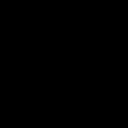
\includegraphics[scale=0.5]{img/black-square.png}
    \caption{Quadrado preto. Fonte: \citeonline{tortinhas}.}%
    \label{fig:f1}
\end{figure}



\section{Resultados}%
\label{sec:resultados}


\section{Conclusão}%
\label{sec:conclusao}

% =====

% =====
% ELEMENTOS PÓS-TEXTUAIS
% =====
\postextual{}

% --- Referências ---
\bibliography{bibliography}

% --- Glossário ---
\printglossary[type=main,style=altlist,title=Glossário]
\printglossary[type=acronym,style=altlist,title=Lista de Abreviaturas e Siglas]
% =====

\end{document}